\title{Survivable Set Connectivity}
\author{
 by Fermi Ma and Erik Waingarten
}
\date{\today}

\documentclass[12pt]{article}
\usepackage{amsmath}
\usepackage{amsthm}
\usepackage{amsfonts}
\usepackage{graphicx}
\usepackage{clrscode4e}
\usepackage{geometry}
 \geometry{
 a4paper,
 total={210mm,297mm},
 left=20mm,
 right=20mm,
 top=20mm,
 bottom=20mm,
 }

\newtheorem{proposition}{Proposition}
\newtheorem{definition}{Definition}
\newtheorem{lemma}{Lemma}
\newtheorem{theorem}{Theorem}

\begin{document}
\maketitle

\section{Introduction}

\subsection{Overview}

In this paper, we analyze the problem of Survivable Set Connectivity (SSC), a generalization of the classical Set Connectivity problem. Set connectivity is formulated as:
\begin{quote}
\textbf{Input}: A weighted graph $G = (V, E)$, with edge cost function $c: E \rightarrow \mathbb{R}^{\geq 0}$ and a collection of $h$ tuples of the form $(S_i, T_i)$. Each $(S_i,T_i)$ is a pair of disjoint vertex subsets. \\
\textbf{Output}: A minimum cost subgraph $H \subseteq G$ such that there is a path between $S_i$ and $T_i$ for each $i$. 
\end{quote}

Note that a ``path between $S_i$ and $T_i$" refers to any path that connects a vertex in $S_i$ to a vertex in $T_i$. The cost of a subgraph is simply the sum of the cost of the subgraph edges.

In SSC, the problem is modified so that each pair of sets $(S_i,T_i)$ must be connected by $k_i$ paths, instead of just 1. More formally, the problem is:

\begin{quote}
\textbf{Input}: A weighted graph $G = (V, E)$, with edge cost function $c: E \rightarrow \mathbb{R}^{\geq 0}$ and a collection of $h$ tuples of the form $(S_i, T_i)$, along with a value $k$. Again, each $(S_i,T_i)$ is a pair of disjoint vertex subsets. \\
\textbf{Output}: A minimum cost subgraph $H \subseteq G$ such that there are $k$ edge-disjoint paths between $S_i$ and $T_i$ for each $i$. 
\end{quote}

Unfortunately, even approximating Survivable Set Connectivity is $\mathsf{NP}$-hard \cite{ssc}. Therefore, the focus of this paper is on an approximate solution to a relaxation of this problem given in \cite{ssc}. Instead of requiring at least $k$ edge-disjoint paths between each pair, we require that each pair have at least $\Omega(\frac{k}{\log n})$ edge-disjoint paths, where $n = |V|$. With this relaxation, it is possible to find a subgraph with cost $O(polylog(n))$ times the optimum.

The paper is organized as follows. Sections 2, 3, and 4 provide the background necessary to understand the algorithm by Chalermsook et al. In Section 2, we present a natural integer linear programming formulation of the problem. Then, in Section 3, we introduce the idea of a \emph{tree embedding}, which allows us to transform arbitrary graphs $G$ into trees that can be more easily handled by the algorithm. In Section 4, we give a rounding scheme by Garg et al. known as RoundGKR, which the algorithm uses as a black box \cite{GKR}. We then pull together these concepts in Section 5 to present the approximation algorithm for SSC by Chalermsook et al. Finally, in Section 6, we analyze the performance of the algorithm.

\subsection{Related Work and Context}

The paper by Chalermsook et al. is the first and (currently) only paper to consider the Survivable Set Connectivity problem \cite{ssc}. Therefore, we survey the only known approximation algorithm for the problem. Chalermsook et al. noted that the original Set Connectivity problem has a large body of prior work, but they found that the best techniques for solving Set Connectivity do not translate to the survivable variant of the problem. Thus, we present Survivable Set Connectivity as a standalone problem, despite its obvious similarities to Set Connectivity.

At this time, it seems that Survivable Set Connectivity is motivated primarily by theoretical interest, as a ``natural" generalization of Set Connectivity. It is unknown if any common real-life graph problems are naturally formulated as a Survivable Set Connectivity problem.

\section{An Integer Linear Program}

In this section, we give an integer linear program that exactly solves SSC. Recall that the goal is to output a subgraph $H$ of $G$ such that each $(S_i,T_i)$ pair has at least $k$ edge disjoint paths. Naturally, we create an indicator variable $x_e$ for each edge based on whether or not it is included in $H$. 
\begin{align}
 x_e &= \left\{ \begin{array}{cc} 1 & e \in H \\
                                  0 & \text{ otherwise. } \end{array} \right.
\end{align}
Thus, our output $H$ will be the subgraph consisting of edges $e$ where $x_e = 1$. Also, for a graph $G = (V,E)$ and for a set $S \subseteq V$, we define $\delta(S)$ to be the set of edges crossing the cut from $S$ to $V \setminus S$. 
With this setup, we claim that the following ILP captures SSC exactly. 
\begin{align}
\min & \sum c(x) x_e  \\
\text{ s.t } & \sum_{e \in \delta(S)} x_e \geq k, \text{for each }S\text{ where } S_i \subset S,T_i \subset V \setminus S,  \\
& x_e \in \{0,1\} \text{ for all }e \in E
\end{align}

The objective function $\sum c(x) x_e$ simply minimizes the cost of all edges included in $H$. The constraint ensures that for all pairs $(S_i,T_i)$, any cut where $S_i$ is on one side of the cut and $T_i$ is on the other side has at least $k$ edges crossing the cut. This property holds if and only if there are $k$ edge disjoint paths from $S_i$ to $T_i$. 

Of course, since this is an integer linear program, our best hope is to approximate it. We relax the program to fractional solutions, so the constraint that $x_e \in \{0,1\}$ becomes $0 \leq x_e \leq 1$. However, there is still a slight issue; we have exponentially many constraints. This occurs because there can be exponentially many choices of $S$ for each $(S_i,T_i)$ pair. To get around this issue, we note that the ellipsoid algorithm can handle linear programs with arbitrarily many constraints, as long as it is given a polynomial time separation oracle. Luckily, such an oracle exists and we sketch it here.

The oracle computes the minimum $S_i, T_i$ cut in the graph. It contracts $S_i$ and $T_i$ to single vertices, and then computes the min-cut in the remaining graph. If there is a min-cut of size less than $k$, then that cut will correspond to a violating contraint. If the min-cut has size at least $k$, then all cuts have size at least $k$, so all constraints are satisfied.

%The next tool we will need are tree embeddings. We have seen metric embeddings in class. Basically, we had a desired type of object $O$ (in the case of cuts, we had a metric space corresponding to a cut) what we did was come up with a metric space $(X, d)$ and a map $f: (X, d) \rightarrow O$ such that the map satisfied certain properties on the distances. 
%
%Here we will have a similar goal. We want to understand minimum cost weighted graphs, but since analyzing them is hard, we instead study minimum cost weighted trees, and then we map the trees back to the graphs. 
%
%\begin{definition}
%A tree embedding of a weighted graph $G = (V, E)$ will be a tree $T = (V_T, E_T)$ with weights $y: E \rightarrow \mathbb{R}^{\geq 0}$ and a function $\text{map} : V_T \cup E_t \rightarrow V \cup P(E)$ ($P(E)$ is the power set of $E$) such that
%\begin{align}
%\text{map}(V_t) &\subset V \\
%\text{map}(E_t) &\subset E
%\end{align}
%In other words, vertices map to vertices and edges map to edges. We will usually refer to an embedding as $(T, y, \text{map})$. 
%\end{definition}

\section{R\"{a}cke's Trees}
\label{sec:rackestrees}

In this section, we introduce a specific type of \emph{tree embedding}. A tree embedding is a transformation that takes general graphs and maps them to trees, while preserving specific information present in the original graph. This way, algorithmic techinques that work well on trees can be applied to general graphs after a tree embedding has been applied. 

For the SSC problem, we will use a specific tree embedding formulated by R\"{a}cke, known as R\"{a}cke's trees \cite{racke}. The property we are most interested in is the way that R\"{a}cke's tree embeddings preserve flow properties in the original graph. The definition of these embeddings is as follows. (\emph{Note to the reader:} the following definitions are quite long, so it may be helpful to reference Figure 1 on the following page while reading the definitions.)

\begin{definition}
For a given graph $G = (V, E)$ with edge capacities $x_e \geq 0$ for all $e \in E$, a R\"{a}cke's Tree embedding is a triple of the form $(T,y,\mathrm{map})$ where $T = (V_T,E_T)$ is a rooted tree, $y$ is a capacity function on the edges $E_T$ (with $y_e \geq 0$ for all $e \in E_T$), and $\mathrm{map}$ is a function that maps vertices in $V_T$ to vertices in $V$, and edges in $E_T$ to sets of edges in $E$. The following properties must also hold:
\begin{enumerate}
\item For each node $v \in V_T$, $\mathrm{map}(v) \in V$. Furthermore, $\mathrm{map}$ restricted to the leaves of $T$ is a bijective function whose image contains all vertices of $G$. In other words, each leaf of the tree $T$ is in one-to-one correspondence with a vertex of the original graph, $G$.
\item For each edge $e = (u,v) \in E_T$, $\mathrm{map}(e)$ is a set of edges that form a path between $\mathrm{map}(u)$ and $\mathrm{map}(v)$. Note that $\mathrm{map}(u)$ and $\mathrm{map}(v)$ are vertices in $G$, so $\mathrm{map}(e)$ specifies a set of edges in $G$.
\item The edge capacities, $y_e$, must be set by the following procedure: The removal of $e$ from $T$ separates the tree into two connected components. Let $S$ be the set of vertices of $G$ mapped to by the leaves of one of the connected components, and so $V \setminus S$ is the set of vertices of $G$ mapped to by the leaves of the other connected component. Recall that $\delta(S)$ is the set of edges in $E$ that cross from $S$ to $V \setminus S$. Then we set $y_e = \sum_{e' \in \delta(S)} x_{e'}$, the total edge capacity crossing the cut.
\end{enumerate}
\end{definition}

We point out a small possibility for confusion here. We think of a R\"{a}cke's tree embedding as a transformation from a graph to a tree, but the $\mathrm{map}$ function used in the above definition is a function from the tree to the graph. Thus, the function that actually \emph{embeds} the graph into the tree is the inverse function, $\mathrm{map}^{-1}$.

Thus, we clarify the properties of $\mathrm{map}^{-1}$. If we apply $\mathrm{map}^{-1}$ to a node in the original graph, $v \in V$, we note that multiple vertices in $T$ could map to $v$. Thus, we specify that $\mathrm{map}^{-1}(v)$ be the unique \emph{leaf} vertex in $V_T$ that maps to $v$. Recall that this uniqueness follows from the bijection property outlined in the above definition. We also consider $\mathrm{map}^{-1}$ applied to sets of vertices $W \subseteq V$, and we define it in a natural fashion: $\mathrm{map}^{-1}(W) = \bigcup_{v \in W} \mathrm{map}^{-1}(v)$.

For edges in the original graph, $e \in E$, we define $\mathrm{map}^{-1}(e) = \{ f \in E_T | e \in \mathrm{map}(f)\}$. This is simply the set of all edges $f$ in the tree $T$ that get mapped to a set of edges $\mathrm{map}(f) \subseteq E$ that contain $e$. Again, this definition can be extended to sets of edges $F \subseteq E$, so that $\mathrm{map}^{-1}(F) = \bigcup_{e \in F} \mathrm{map}^{-1}(e)$.

At this point, we direct the reader to Figure 1, which contains a visualization of the above definitions.

The usefulness of R\"{a}cke's trees becomes apparent when we consider multi-commodity flows. Recall that the multi-commodity flow problem specifies $k$ different commodities, where each commodity $i$ must be routed from source $s_i$ to sink $t_i$, subject to constraints on the capacity of each edge. The resulting flow can be represented as a set of functions $\{ f_i \}$, where $f_i(e)$ is the nonnegative real number amount of commodity $i$ flowing on edge $e$. 

There is a natural way to map multi-commodity flows between $G$ and $T$. In particular, suppose we have a multi-commodity flow $\{ f_i \}$ on $G$. For each $i$, if there are $f_i$ units of flow going from $s_i$ to $t_i$ in $G$, we route $f_i$ units of flow in the $T$ from $\mathrm{map}^{-1}(s_i)$ to $\mathrm{map}^{-1}(t_i)$. For the other direction of the mapping, suppose we are given a multicommodity flow $\{ f_i^T \}$ in $T$. If edge $e \in T$ has $f_i^T(e)$ units of flow, then we route $f_i^T(e)$ units of flow through the path $\mathrm{map}(e)$ in $G$ (recall that edges in $T$ map to paths in $G$).

\begin{figure}
\label{fig:racketree}
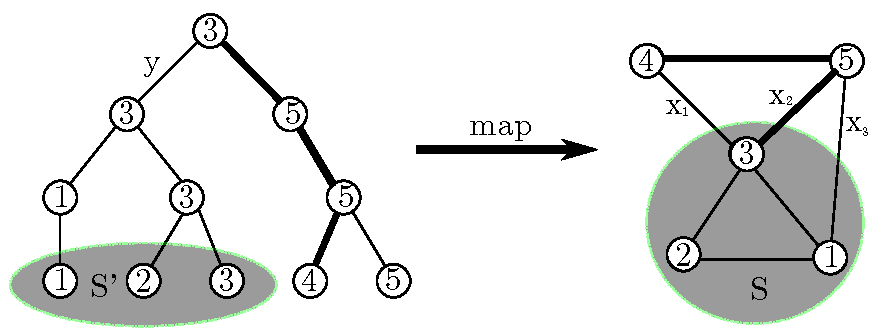
\includegraphics[width=\linewidth]{RackeTree.pdf}
\caption{An example of a R\"{a}cke's tree embedding. On the left, we have the tree $T$, and on the right, we have the original graph $G$ which is embedded in $T$. Nodes of $G$ are labeled from 1 through 5, and the nodes of $T$ are labeled by the nodes of $G$ that they are mapped to. Note in particular that the leaves of $T$ contain all the labels from 1 through 5, as there is a bijection between the tree leaves and the graph nodes. In addition, observe that multiple nodes of the tree map can map to the same node in the graph. For example, four nodes in the tree all map to node 3 in $G$, but we specify that $\mathrm{map}^{-1}(3)$ be the specific leaf node that maps to 3.
\newline
\text{ }\hspace{.3in} Consider the edge labeled $y$ in the tree. The removal of $y$ separates the leaves of the tree into those that are in $S'$ and those that are not in $S'$. The leaves in $S'$ map to the nodes in $S$ in $G$, and so the capacity of $y$ is given by the sum of the capacities of the edges that span the cut $(S,V\setminus S)$. These edge capacities are $x_1$, $x_2$, and $x_3$, so the capacity of $y$ is $x_1 + x_2+x_3$.
\newline
\text{ }\hspace{.3in} Certain edges are bolded to highlight the effect of $\mathrm{map}$ on edges. Since the $\mathrm{map}$ function maps edges in the tree to paths in $G$, we have that the bolded edge from 3 to 5 in the tree maps to the bolded length 1 path from 3 to 5 in the graph. The bolded edge from 5 to 5 maps to the empty path of length 0 from 5 to 5 in the graph. The bolded edge from 4 to 5 maps to the bolded path of length 1 from 4 to 5 in the graph.}
\end{figure}

We define the distribution $\mathcal{D}$ as the uniform distribution over all possible R\"{a}cke's tree embeddings for a given graph $G$. There is a polynomial time algorithm for sampling from this distribution, given in \cite{racke}. This distribution $\mathcal{D}$ will be important for describing the SSC algorithm, as the algorithm will sample from it.\\

Lastly, we introduce the idea of load.

\begin{definition}
Given a R\"{a}cke's tree, the load on an edge of the graph $e \in E$ is
\begin{align}
load(e) &= \sum_{f \in \text{map}^{-1}(e)} y_f,
\end{align}
\end{definition}
We can also define the relative load, $rload(e) = load(e)/x_e$.

We provide intuition behind the definition of load. Note that in Figure 1, $load(x_1) = 0$, since $\mathrm{map}^{-1}(x_1) = \emptyset$. As an immediate consequence of this, we can see that removing an edge with load 0 does not affect the connectivity of the graph. At a high level, the load measures how necessary an edge is for connectivity. \\
\noindent \textbf{Additional Details.} For the remainder of this section, we provide a number of statements regarding R\"{a}cke's trees that will be applied to complete the analysis of the algorithm in Section 6. They are provided here for the sake of completeness, but the reader may skip this section and refer to it if interested while reading the proofs in Section 6.

The following lemmas are due to R\"{a}cke, and we state them without proof. Their proofs can be found in \cite{racke}.

\begin{lemma}[\cite{racke}]
\label{lem:mapflows}
If we have a graph $G = (V, E)$ and capacities $x: E \rightarrow \mathbb{R}^{\geq 0}$ and a Racke tree $(T, y, \text{map})$. A multicommodity flow on $G$, $\{ f_i \}$, maps directly to a multicommodity flow on the tree which is also feasible. Likewise, a multicommodity flow on $T$ maps directly into a multicommodity flow on the graph, with the small caveat that we must multiply the capacity of the edge by the relative load. 
\end{lemma}

\begin{lemma}[\cite{racke}]
\label{lem:rload}
For some given graph $G = (V, E)$ and capacities $x: E \rightarrow \mathbb{R}^{\geq 0}$, we can sample efficiently from R\"{a}cke's trees of $G$, such that 
\begin{align}
\max_{e \in E} \textbf{E}[rload(e)] &\leq \alpha = O(\log n) 
\end{align}
\end{lemma}

\begin{lemma}[\cite{ssc}]
\label{thm:height}
The height of the trees sampled is $O(\log nC)$, where $C$ is the ratio of the largest to smallest capacity in $G$. In our cases, the height will always be $O(\log n)$. 
\end{lemma}


\section{The RoundGKR Procedure}

The final component we need for the SSC algorithm is the RoundGKR procedure, named for its inventors, Garg, Konjevod, and Ravi \cite{GKR}. This is the rounding procedure the algorithm for SSC uses, and we will see that this rounding procedure only works for trees. We introduced tree embeddings in the previous section solely because of this fact. Originally, RoundGKR was developed for the Group Steiner Tree (GST) problem. In order to explain the procedure, we give a brief overview of the problem. \\

Group Steiner Tree:
\begin{quote}
\textbf{Input}: A tree $T = (V_T, E_T)$ rooted at $r$ where each edge has a nonnegative real value cost $c(e)$, along with with a collection of sets $T_i$ where each $T_i \subseteq V_T$.\\
\textbf{Output}: The minimum cost subtree $H \subseteq T$ with a path from $r$ to $t_i$ for some $t_i \in T_i$ for all $i$.
\end{quote}

The following integer linear program solves the problem exactly:
\begin{align}
\min & \sum c(e) y_e  \\
\text{ s.t } & \sum_{e \in \delta(S)} y_e \geq 1, \text{ where } S_i \subset S, T_i \subset V - S\\
&y_e \in \{0,1\}
\end{align}

Recall that $\delta(S)$ is the set of edges spanning the cut $(S,V_T \setminus S)$. This program is almost identical to the program for Survivable Set Connectivity, but with $k$ replaced with 1. The argument for why this program works is the same as before; we are minimizing the total cost of the included edges, and we are ensuring with the constraints that there is a path from $r$ to $t_i$ for some $t_i \in T_i$.

If we relax the integer linear program to a linear program and solve it, we can use RoundGKR to round the resulting fractional solution to an integer solution. The optimum to the linear program will assign fractional values in $[0,1]$ to each $y_e$. For any $e$, let $p(e)$ denote its parent edge in the tree (if it exists). We claim that since our problem is to find a subtree that includes the root $r$, edges that are closer to the root are at least as likely to be included in the subtree than edges farther from the root. Since the value of $y_e$ will be used as the probability that edge $e$ is included in $H$, we will assume that $y_{p(e)} \geq y_e$. 

The RoundGKR procedure simply starts at the root $r$ and builds the subtree $H$ by working its way down the original tree, $T$. It decides whether or not to include edge $e$ only once it has included edge $p(e)$ (if ever). At this step, it includes $e$ with probability $\frac{y_e}{y_{p(e)}}$. A simple inductive argment shows that an edge $e$ is chosen with probability $y_e$ (proof sketch: assume by induction that we know $Pr[\text{include $p(e)$}] = y_{p(e)}$. Then $Pr[\text{include $e$}] = Pr[\text{include $e$ $|$ include $p(e)$}]*Pr[\text{include $p(e)$}] = \frac{y_e}{y_{p(e)}}y_{p(e)} = y_e$.)

The most important property of RoundGKR is the following lemma, whose proof can be found in \cite{GKR}.

\begin{lemma}[\cite{GKR}]
\label{lem:findpath}
Suppose that $T = (V_t, E_t)$ supports a flow of at least $1$ from $T_i$ to the root $r$ without using some set of edges $F_t$. Then RoundGKR returns a solution with a path in $T$ from $T_i$ to $r$ without using $F_t$ with probability at least $\Omega(\frac{1}{\log n})$. 
\end{lemma}
%
%We will rely on this lemma heavily. In fact, since we need $\Omega(\frac{k}{\log n})$ edge-disjoint paths, we will argue that if we let $F_t$ be any set of at most $\Omega(\frac{k}{\log n})$ edges, then we still have a path, and therefore, we have $\Omega(\frac{k}{\log n})$ paths.  

\section{Algorithm}

In this section, we present the approximation algorithm given by Chalermsook et al \cite{ssc}. The algorithm uses many concepts presented earlier in the paper, which we remind the reader of first.

The algorithm takes as input a graph $G = (V,E)$ with edge cost function $c$ and $h$ tuples of the form $(S_i,T_i)$ along with a value $k$. The algorithm outputs a subgraph $H \subseteq G$, represented as a set of edges of $G$, such that there are at least $\Omega(\frac{k}{\log n})$ edge-disjoint paths between $S_i$ and $T_i$ for each $i$. Recall that $k$ edge-disjoint paths was the goal, so we fall short of this requirement by a logarithmic factor. The cost of $H$, equal to the sum of the edge costs in $H$, is within a polylogarithmic factor of the optimum. 

Recall that SSC-LP is the linear programming relaxation of the ILP for SSC, presented in Section 2. Also, $\mathcal{D}$ is the distribution over all possible R\"{a}cke's tree embeddings for a graph $G$, which we can sample from in polynomial time. In the algorithm, we use the variable $\tau$ set to be $\log(h)+k$, $\tau'$, set to be $O(\log n)$, and $q$ as an index. The algorithm is as follows.

\begin{codebox}
\li Set $H \leftarrow \emptyset$
\li Compute linear program SSC-LP and set to zero any $x_e < \dfrac{k}{n^2}$.
\li Let $x' \leftarrow x*\frac{4}{k}$. 
\li Let $\mathcal{D}$ be the distribution of R\"{a}cke's tree embeddings for $G$ with $x'$.
\li \For $\tau$ rounds \Do
\li Sample $(T, y, \text{map})$ from $\mathcal{D}$. 
\li \For $q = 0, ..., 2\log n$ \Do
\li \For $v \in V_t$ \Do
\li With probability $\min\{1, \dfrac{4}{2^q}\}$, $q$-mark $v$
\li \If $v$ is $q$-marked \Then
\li Set $y^{v, q}\leftarrow 2^{q+1}y$ and $E^{v,q} \leftarrow \emptyset$.
\li \For $\tau'$ iterations, \Do
\li $E^{v,q} \leftarrow E^{v,q} \cup$ RoundGKR$(T_v, v, y^{v,q})$ \End
\li $H \leftarrow H \cup \text{map}(E^{v,q})$ \End \End \End \End
\li return $H$
\end{codebox}

\subsection{Algorithm Idea}

Here, we provide an intuitive explanation of the algorithm as well as the main motivations for each procedure. Of course, we will revisit these ideas in the analysis.

The algorithm first solves the linear programming relaxation, which produces a value of $x_e \in [0,1]$ for each edge $e \in E$. The first step is to zero out all values of $x_e < \frac{k}{n^2}$. After this, the values are scaled down from $x$ to $x'$ by a $\frac{4}{k}$ factor. Since the linear progrom ensures a fractional path of total capacity $k$ from $S_i$ to $T_i$ for each $i$, this $4/k$ scaling ensures fractional paths of total capacity $4$. Since we argued that a flow in the original graph $G$ corresponds to a flow of the same value in any corresponding R\"{a}cke's tree, the resulting tree embeddings will also have flows of value 4. 

The next step, which the algorithm repeats $\tau = \log(h) + k$ times, begins by sampling a random R\"{a}cke's tree embedding for the graph $G$. Then, we create an index $q$ which scrolls from 0 to $2\log n$. For each vertex of the tree embedding, and for all possible values of the index $q$, we perform an operation called $q$-marking. This simply involves labeling each vertex with the values of $q$ that we $q$-mark it with. Therefore, any given vertex can be $q$-marked up to $2\log n + 1$ times. For each value of $q$, we $q$-mark a given vertex with probability $\min\{1, \dfrac{4}{2^q}\}$. Then for each vertex $v \in E_T$, we go through all values of $q$ such that $v$ was $q$-marked and perform the following steps: 1) Create a new capacity function $y^{v,q}$ that is the original capacity function $y$ for the tree embedding, scaled up by a factor of $2^{q+1}$. 2) Initialize the set $E^{v,q}$ to be empty. 3) For $\tau' = O(\log n)$ iterations, run the RoundGKR procedure on the R\"{a}cke's tree, with the given capacity function $y^{v,q}$. Whenever edges are output by the procedure, we add them to $E^{v,q}$.

The purpose of these scaling constants is to ensure that the RoundGKR procedure, which looks for paths of value 1, will actually see these paths. We preserve the fact that paths with low capacity are chosen with lower probability. The reason why we have $\tau' = O(\log n)$ iterations is because is because  Lemma~\ref{lem:findpath} shows that RoundGKR finds paths in trees which avoid specific edges with probability $\Omega(\frac{1}{\log n})$. $O(\log n)$ repetitions ensure a constant probability of finding such paths.

Finally, the algorithm concludes by spitting out all of the edges ever returned by any RoundGKR procedure run on any of the iterations for any of the values of $q$ for any of the nodes $v$ that are $q$-marked.
%
%Lemma~\ref{lem:findpath} requires us to have a flow of at least $1$ avoiding some edges. If a flow path from $s_i'$ to $t_i'$ goes through ancestor $v$ and carries a flow of value $f$, we can apply the lemma if $f \geq 1$. We scale the capacities by $2^{q+1}$ in order to search for the flow value. We only scale with probabilities $\dfrac{4}{2^q}$ so our costs does not increase by more than $O(\log n)$. Figure~\ref{fig:roundgkronnode} shows how a flow path might be found.

\section{Algorithm Analysis}

\subsection{Overview}

We claim that the algorithm finds a solution which has
\begin{itemize}
\item (Claim A) cost within a polylogarithmic factor of the optimum
\item (Claim B) at least $\Omega(\frac{k}{\log n})$ edge disjoint paths between each $(S_i, T_i)$ pair
\end{itemize}

We first prove Claim A assuming that Claim B is true, and then we prove claim B.


\subsection{Claim A}

\begin{lemma}[\cite{ssc}]
\label{lem:cost}
$\textbf{E}[c(H)] = O(\log^4n(\frac{\log h}{k}+1)) * c(x)$, where $c(x) = \sum_e c(e)x_e$. 
\end{lemma}

Observe that $c(x)$ is the value of the LP-optimum, which must be at least as good as the true optimum of the problem. Therefore, this lemma shows that the cost of the algorithm's solution is within an $O(\log^4n(\frac{\log h}{k}+1))$ factor of the optimum.

\begin{proof}
We prove this by bounding the probability that a given edge is included in $H$ by $O(\log^4n(\frac{\log h}{k} + 1))x_e$. The claim then follows by linearity of expectation.

Let $(T = (V_T, E_T), y, \text{map})$ be a R\"{a}cke's tree sampled from $\mathcal{D}$. For an edge $e$ to be included in our output subgraph $H$, there must have been some tree edge $e' \in E_T$ that maps to $e$ (so $e \in \mathrm{map}(e')$) selected to be in $E^{v,q}$ for some vertex $v \in V_t$ and some index $q \in [0,\dots,2\log n]$. For this to occur, $v$ must be $q$-marked, an event that occurs with probability $\frac{4}{2^{q}}$. 

We first bound the probability that an edge $e' \in E_T$ is included, which we will then use to bound the probability the algorithm includes an edge $e \in E$.

For a given edge $e' \in E_T$, there are at most $height(T)$ ancestors, which means that there are at most $height(T)$ different vertices $v$ that, if $q$-marked, may lead to $e'$ being included. For each $v$, we must consider all $O(\log n)$ possible values of $q$. For each value of $q$, the probability of being $q$-marked is $\frac{4}{2^{q}}$. Once the vertex is $q$-marked, we have $\tau'$ trials of the RoundGKR algorithm, where in each trial, there is a $2^{q+1}y_{e'}$ chance of edge $e'$ being included (by construction of the algorithm). Multiplying these probablities together and applying a union bound over all $\tau'$ trials and over all possible values of $q$, we get an upper bound of 

\begin{align}
height(T) \sum_{q=0}^{2\log n} \frac{4}{2^{q}} 2^{q+1} y_{e'} \tau' &= height(T) \tau' y_{e'} \sum_{q=0}^{2\log n} 8 = O(\log^3 n) y_{e'} 
\end{align}

So the probability that a given edge of the tree is included in a particular sampling of a R\"{a}cke's tree is $O(\log^3 n) y_{e'}$. 

Using this, we can bound the probability that a particular edge $e$ of the original graph is included. For $e$ to be included, on one of the $\tau$ trials, the algorithm must chose some tree edge $e'$ such that $e' \in \mathrm{map}^{-1}(e)$ (recall that this is the set of tree edges which, if selected, result in edge $e$ being included). So let $X_e$ be the indicator random variable which says that edge $e$ is included in $H$. Then we have the inequality
\begin{align}
 \textbf{E}_{R}[X_e] &\leq \tau \sum_{e' \in \mathrm{map}^{-1}(e)} O(\log^3 n) y_{e'} 
\end{align}
where the expectation $\textbf{E}_{R}[X_e]$ is over the random choices of the algorithm, after choosing a R\"{a}cke's tree. The $\tau$ comes from a union bound over all trials. The $O(\log^3 n)y_{e'}$ comes from the first part of the proof, where we bounded the probability of including a specific $e'$. 

The remainder of this proof relies heavily on the definitions and lemmas stated at the end of Section 3. We apply those results in order to simplify the inequality we have above and get our final result. We first take the expectation over the random choice of drawing a R\"{a}cke's tree from the distribution $\mathcal{D}$. This gives
\begin{align}
\textbf{E}_{\mathcal{D}}[E_{R}[X_e]] &\leq \textbf{E}_{\mathcal{D}}[\tau \sum_{e' \in \mathrm{map}^{-1}(e)} O(\log^3 n) y_{e'}] \\
               &\leq O(\log^3 n) \tau \textbf{E}_{\mathcal{D}}[\sum_{e' \in \mathrm{map}^{-1}(e)} y_{e'}]
\end{align}

Recall that in Section 3, we defined $load(e) = \sum_{e' \in \mathrm{map}^{-1}(e)} y_{e'}$ and $rload(e) = load(e)/x_e$. We thus rewrite the inequality as
\begin{align}
              \textbf{E}_{\mathcal{D}}[E_{R}[X_e]]  & \leq O(\log^3 n) \tau \textbf{E}_{\mathcal{D}}[load(e)]\\
&\leq O(\log^3 n) \tau \textbf{E}[rload(e) x_e'] \\
                &\leq O(\log^3 n) \tau \frac{4}{k} \alpha x_e
\end{align}
The last line of the above computation uses the value of $\alpha$, defined in Section 3 as $\alpha = max_{e \in E}\textbf{E}[rload(e)]$. We have from Lemma 2 that $\alpha$ is $O(\log n)$. To simplify notation, we write $\textbf{E}[X_e]$ as the expectation over both random choices of the algorithm as well as random choices of the R\"{a}cke tree. So our final inequality is 
\begin{align}
 \textbf{E}[X_e] &\leq \frac{O(\log^4 n)\tau}{k} x_e 
\end{align}

From here, we simply apply linearity of expectation to bound the total cost. We have 
%
%
% Above, we argued that $E[Y_{e'}] \leq O(\log^3 n)y_{e'}$.
%\begin{align}
%X_e \leq \sum_{e' \in \text{map}(e)} Y_{e'}
%\end{align}
%Because if $e$ is included in the graph, it must have come from some edge in the tree. 
%\begin{align}
% \textbf{E}[X_e] &\leq \tau \sum_{e' \in \text{map}^{-1}(e)} O(\log^3 n) y_{e'} \\
%        &= O(\log^3 n) \tau \textbf{E}[load(e)] \\
%        &= O(\log^3 n) \tau \textbf{E}[rload(e)x_e'] \\
%        &\leq O(\log^3 n) \tau \dfrac{4}{k} \alpha x_e\\
%        & = \dfrac{O(\log^4 n)\tau}{k} x_e
%\end{align}
%So now, bounding the optimum, we get
\begin{align}
\textbf{E}[c(H)] &= \sum_{e \in E} c(x_e)\textbf{E}[X_e] \\
                 &\leq \dfrac{O(\log^4 n)\tau}{k} \sum_{e \in E} c(x_e) x_e
\end{align}
So when $\tau = O(\log h + k)$, we get our desired approximation.
\end{proof}
%
%\begin{figure}
%\label{fig:roundgkronnode}
%\centering
%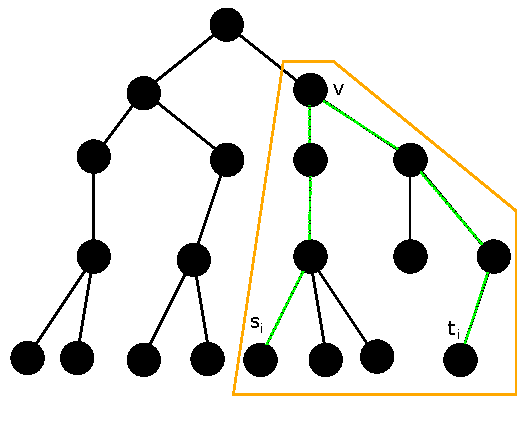
\includegraphics[width=0.6\linewidth]{RoundGKRonNode.pdf}
%\caption{Execution of GKR on some subtree rooted at $v$ in a particular round finding paths to $s_i$ and $t_i$.}
%\end{figure}

Having established that the expected cost is only a polylogarithmic factor away from the optimum, it remains to show that the edges chosen do in fact form a graph which connects $(S_i, T_i)$ with $\Omega(\frac{k}{\log n})$ disjoint paths for each $i$. We prove this in the next section.

\subsection{Claim B}

First, we define a notion of \emph{good} and \emph{bad} tree embeddings with respect to a subset of edges $F \subseteq E$.


\begin{definition}
For a set of edges $F \subseteq E$, let $F_T = \text{map}^{-1}(F)$. Then a R\"{a}cke's tree embedding is bad for $F$ if 
\[ \sum_{e' \in F_T} y_{e'} \geq \frac{1}{2} \]
And good otherwise.
\end{definition}

Intuitively, if a tree embedding is bad with respect to a set $F$, then $F$ is necessary for connectivity in the graph. For our argument, we will want tree embeddings to be good with respect to sets of size $\Omega(\frac{k}{\log n})$ in order to ensure connectivity even if these sets are removed.

\begin{lemma}[\cite{ssc}]
\label{lem:notbad}
Fix some $F$ of size at most $\dfrac{k}{16 \alpha}$. Then the probability that a sampled tree embedding $(T, y, \text{map})$ from $\mathcal{D}$ is bad is at most $\frac{1}{2}$. 
\end{lemma} 

\begin{proof}
Suppose we have a bad embedding for the set $F$. Using the definition of load, we write
\begin{align}
\sum_{e \in F} load(e)&= \sum_{e \in F} \sum_{e' \in \text{map}^{-1}(e)} y_{e'} \\
                    &\geq \sum_{e' \in F_T} y_{e'} \\
                    &\geq \frac{1}{2}
\end{align}
where the first inequality arises from comparing a sum over a union to a sum over a disjoint union (summands in the first line are counted at least as many times as summnds on the second line), and the second inequality from the assumption that the tree embedding is bad for F.

Therefore, a bad tree means that the load of the set of $F$ (shorthand for the sum of the loads of the edges in $F$) is more than $\frac{1}{2}$. Therefore,
\begin{align}
Pr[\text{pick a bad tree for $F$}] &\leq Pr[ \sum_{e\in F} load(e) \geq \frac{1}{2}]
\end{align}
From Lemma~\ref{lem:rload}, we know that
\begin{align}
\textbf{E}[ \sum_{e \in F} load(e) ] &\leq \sum_{e \in F} \textbf{E}[rload(e)]x_{e'} \\
                                   & \leq \sum_{e\in F} \alpha \frac{4}{k} x_{e} \\
                                   & \leq \dfrac{4\alpha}{k} |F| \\
                                   &\leq \frac{1}{4}
\end{align}
where the last inequality comes from our assumption about the size of $F$. Invoking Markov's inequality, the probability that the sum of the loads exceeds $1/2$ is at most $1/2$, so the probability of a bad event is at most $\frac{1}{2}$. 
\end{proof}

Now, we can state the theorem we need for the desired connectivity claim. Note that since $\alpha = O(\log n)$, the following result says that between each $S_i$ and $T_i$, we have $\Omega(\frac{k}{\log n})$ paths.

\begin{theorem}[\cite{ssc}]
\label{theorem:connected}
With probability at least $\frac{3}{4}$, all set pairs are at least $\frac{k}{16\alpha} + 1$ edge connected in $H$. 
\end{theorem}

As the proof of this theorem is complicated, we break up the overall structure of the proof into five parts.

\textbf{Proof Structure for Theorem~\ref{theorem:connected}}:
\begin{enumerate}
\item Fix a particular set of edges $F \subseteq E$ of size at most $\frac{k}{16\alpha} = \Omega(\frac{k}{\log n})$. 
\item Argue that with probability at most $\frac{1}{2}$, the edges in $F$ are not necessary for graph connectivity by claiming that the total $load$ on the edges in low. (This is Lemma~\ref{lem:notbad}). 
\item Condition on the event of $F$ not being necessary to show that if we remove $\text{map}(F)$ from the tree, we still have sufficient flow from each $S_i$ to $T_i$. Note that any flow paths in the tree must go up the tree to some common ancestor $v$ and then back down. Think of these nodes $v$ as ``turning points".
\item Claim that any turning point $v$ will get $q$-marked for some $q$ and so the RoundGKR algorithm which is rooted at $v$ (recall that we run iterations of the RoundGKR algorithm for any node $v$ that gets $q$-marked) finds a path from $v$ to $S_i$ and from $v$ to $T_i$. We show that this path is found with sufficient probability.
\item We union bound over all possible choices of $F$ and over all $i$ to show that we succeed with constant probability. From this, we conclude that removing any set of size $\frac{k}{16 \alpha}$ does not damage connectivity for any of the $(S_i,T_i)$ pairs, so each pair must be at least $\frac{k}{16\alpha} + 1$-connected.
\end{enumerate}

\begin{proof}[Proof of Theorem~\ref{theorem:connected}]

Step 1 is a trivial set-up step, and step 2 was Lemma~\ref{lem:notbad}. Here, we give the details of step 5.

We fix an $F$ of size at most $\frac{k}{16\alpha}$ and an $i$ and show that $(S_i, T_i)$ are connected with an edge outside of $F$. We show this happens with a probability at least $\beta$, which will be some constant greater than 0. So the probability of failure is $(1-\beta)$. If we repeat this $\tau = \frac{1}{\beta}\ln(4hn^{\frac{k}{16\alpha}}) = O(\log h + k)$ times, then our failure probability goes down to $\dfrac{1}{4hn^{\frac{k}{16\alpha}}}$. So we take the union bound over all of $F$ and over all $i$, so we get probability of failure at most $\frac{1}{4}$.

It remains to show that the probability that we find a path from $S_i$ to $T_i$ without using the edges from $F$ is at least $\beta$. We do this in the following lemma.

(As of this point, it remains to show steps 3 and 4, which we do below.)

\begin{lemma}
Fix some $F$ and some $i$, where $|F| < \dfrac{16k}{\alpha}$. The probability that at round $t$ we find a path from $S_i$ to $T_i$ without using edges from $F$ is at least some constant $\beta > 0$. 
\end{lemma}

\begin{proof}

For this lemma, we give a very extensive proof sketch. The goal is to convince the reader that this claim is true, but since the proof is incredibly detail heavy, we will gloss over some minor points.

We condition on the probability that a sampled tree embedding is good with respect to $F$ at round $t$, which by Lemma~\ref{lem:notbad} is at least $\frac{1}{2}$. Now, set the edge capacities $y$ for edges in $F_T = \text{map}^{-1}(F)$ to be zero in order to avoid picking edges in $F$. 

Note that since we start with a solution to the fractional LP, we assume that $G$ supports a flow of at least $k$. Recall that we reweighed the edge capacities $x$ by $\frac{4}{k}$, so we can support a flow of at least $4$ in the original graph with edge capacities $x'$. By Lemma~\ref{lem:mapflows}, any R\"{a}cke's tree embedding for $G$ will supports a flow from $S_i' = \text{map}^{-1}(S_i)$ to $T_i' = \text{map}^{-1}(T_i)$ of value at least $4$. 

Removing $F$ from the graph removes a total capacity of at most $\frac{1}{2}$, and so we are left with a flow of at least $4 - \frac{1}{2} > \frac{3}{2}$. In particular, we can support a unit flow from $S_i'$ to $T_i'$. That unit flow can be decomposed into paths $P_1, ..., P_z$ (disregard paths with very small amounts of flow $(\leq \frac{1}{2n^2})$). Each flow path goes up from a leaf, turns at some $v$, and then goes down to another leaf. Let $\phi_v$ be the total amount of flow from $S_i'$ to $T_i'$ turning at $v$. 

Since we support a flow of at least $\frac{3}{2}$ and we removed paths with at most $\frac{1}{2n^2}$ flow, we are left with $\sum_{v \in V_t} \phi_v \geq \frac{3}{2} - \dfrac{1}{2n^2}|E_t| \geq 1$ units of flow. 

Now since $\phi_v$ is between $\frac{1}{2n^2}$ and 1, it falls between some $(2^{-q_v-1}, 2^{-q_v}]$ for some $q_v \in \{0, ..., 2\log_2 n\}$. The probability that none of the $v \in V_T$ are $q$-marked exactly at $q_v$ when we have a good embedding is at most $e^{-3/4}$ (which can be proven by a Chernoff bound). The important thing to note is that each time we try to $q$-mark a node, it is an independent event. The expected value of the number of vertices that get $q$-marked at $q_v$ is at least $4$ and we need at least $1$. These values are sums of independent random variables, so we can apply the Chernoff bound.

Conditioning on finding one such $v$, the path gets multiplied by $2^{q_v+1}$ (due to construction of the algorithm). After the scaling, it supports a flow of $1$. Lemma~\ref{lem:findpath} says the path will be included with probability at least $\Omega(\frac{1}{\log n})$ in a single round of RoundGKR. So if we repeat it $\tau'$ times, the probability we do not find the path is $1 - (1 - \Omega(1/\log n))^{\tau'}$. Letting $\tau' = O(\log n)$, we get any constant probability $\epsilon$. Since we need to find both paths from the root to both leaves, we get a failure probability of $2\epsilon$.

So the probability that we find a path outside of $F$ is at least one minus the union bound over failure probabilities. This is $1 - \frac{1}{2} - e^{-3/4} - 2\epsilon > 0$. 
\end{proof}

This concludes steps $3$ and $4$ of the proof idea. This finishes the proof that after running the rounding algorithm, each $(S_i, T_i)$ tuple will have $\Omega(\frac{k}{\log n})$ paths connecting $S_i$ to $T_i$. 

\end{proof}

\section{Conclusion}

In this paper, we introduced the Survivable Set Connectivity problem along with the only known approximation algorithm for it. To present the algorithm, we formulated a linear program for the problem, gave a type of tree embedding for general graphs, and a rounding procedure that works exclusively on trees.

It seems that there is much room for improvements to the algorithm, which currently has a $\log^4(n)$ term in the approximation ratio. In an optional section following this conclusion, we give some of our own ideas for potential improvements. We were able to shave one of the $\log(n)$ factors in a very special case, but we did not think that our improvements were substantial enough to deserve a large section in this paper.

\section{Optional Section: Minor Potential Improvements}

To Prof. Karger: This section is completely optional, and not part of our paper. As a group, we were leaning towards not including it at all, but we wanted to show that we had thought about the algorithm deeply outside of just rewriting it.

There seems to be a trade off in the algorithm between finding flow paths between many groups at once and searching for nodes the flow paths traverse. In the original algorithm, we must iterate through each $v \in V_T$ and run some RoundGKRrounds on its subtree. If there are multiple flow paths from different groups, say $(S_1', T_1')$ and $(S_2', T_2')$ going through $v$, then the original algorithm could find both at once. We could be finding $h$ paths with $O(\log n)$ cost (since running RoundGKR on each subtree makes each edge appear in $O(\log n)$ subtrees). 

If we know $\sum_{i=1}^h |S_i| = S$ is small (the number of sources is small). We can run the algorithm without looking for the nodes where the flow paths turn. In particular, we could treat it as many different instances of the Group Steiner Tree problem. The algorithm would be:
\begin{codebox}
\li Set $H \leftarrow \emptyset$
\li Compute linear program SSC-LP and set to zero any $x_e < \dfrac{k}{n^2}$.
\li Let $x' \leftarrow x*\frac{4}{k}$. 
\li Let $\mathcal{D}$ be the distribution of R\"{a}cke's tree embeddings for $G$ with $x'$.
\li \For $\tau$ rounds \Do
\li Sample $(T, y, \text{map})$ from $\mathcal{D}$. 
\li \For $q = 0, ..., 2\log n$ \Do
\li \For \For $i \in [h]$ and $s \in S_i'$ \Do
\li With probability $\min\{1, \dfrac{4}{2^q}\}$, $q$-mark $s$
\li \If $s$ is $q$-marked \Then
\li Set $y^{s, q}\leftarrow 2^{q+1}y$ and $E^{s,q} \leftarrow \emptyset$.
\li \For $\tau'$ iterations, \Do
\li $E^{s,q} \leftarrow E^{s,q} \cup$ RoundGKR$(T_s, s, y^{s,q})$ \End
\li $H \leftarrow H \cup \text{map}(E^{s,q})$ \End \End \End \End
\li return $H$
\end{codebox}
The main difference lies in line 8. Instead of iterating through all $v \in V_T$ to find where the flow path turns, we take advantage of knowing where the flow begins. We know all flow paths go from $S_i'$ to $T_i'$, so we make $s \in S_i'$ the root of the tree. It is unnecessary to look for where the flow turns. We still have to iterate through $q= 0, ..., 2\log n$, since the flow of at least $1$ between $S_i'$ and $T_i'$ might be divided among different flow paths starting at different nodes in $S_i'$. This gets rid of the $O(\log n)$ factor in the cost because of the height, and adds a factor of $S$.

Theorem~\ref{theorem:connected} still holds since we know exactly where the flow paths must start.

\begin{lemma}
The above algorithm has $\textbf{E}[c(H)] = O(S\log^3 n(\dfrac{\log h}{k} + 1))*c(x)$.
\end{lemma}

\begin{proof}
The proof is the same as the proof of Lemma~\ref{lem:cost}. The only difference is that instead of each edge being included in at most $height(T)$ RoundGKR steps, we include it in at most $S$ RoundGKR steps. 
\end{proof}

Therefore, if $S = o(\log n)$, it is better to run this modified algorithm. Along similar lines, if $\sum_{i \in [h]} |T_i| = T$ is small, then we could compress the R\"{a}cke tree to contain only the leaves we want. If $T = O(\log n)$, then the tree could be compressed to size $O(\log n)$, and so we would find unit flow paths with probability $\Omega(\frac{1}{\log \log n})$. This means we could reduce $\tau'$ to $O(\log \log n)$ and decrease our approximation ratio.

Now the question becomes, can we reduce $S$ to $h$? One possible idea is to join all the nodes in $S_i'$. This would destroy the tree property for RoundGKR, but maybe we can disregard some cycles (at least if we analyzed the case with unit costs on the edges). \cite{ssc} uses RoundGKR and R\"{a}cke trees as black boxes, so maybe there is some hope. If this is possible, then our competitiveness would be $O(h\log^3n(\dfrac{\log h}{k} + 1))$. Now if $h = o(\log n)$, then we would prefer this algorithm.

\bibliography{references}
\bibliographystyle{splncs}

\end{document}